\documentclass[12pt,a4paper]{article}
\usepackage{amsmath,amssymb}
\usepackage{graphicx}
\usepackage{float}
\usepackage{tikz}
\usepackage[english]{babel}
\usepackage[utf8]{inputenc}
\usetikzlibrary{shapes, arrows, positioning}


\usepackage{amsmath,amssymb,mdframed}            % AMS package gives better equation layouts
\setcounter{page}{2}                    % sets first page number to 2
\setlength{\oddsidemargin}{-0.25in}     % set left margin
\setlength{\textwidth}{6.5in}           % set text width
\setlength{\topmargin}{-0.5in}          % controls layout at
\setlength{\headsep}{1cm}             % top of page
\setlength{\textheight}{9.0in}          % set text length



\makeatletter
\renewcommand{\@oddhead}{\hfill MA3600/15R}  % sets header
\renewcommand{\@oddfoot}{\hfil \arabic{page} \hfil}    % sets page footer
\makeatother

\renewcommand{\labelenumi}{\arabic{enumi}} % Sets the first level of enumerate to be arabic (normal) numbers
\renewcommand{\labelenumii}{(\alph{enumii})} %Sets the second level of enumerate to be (a), (b), (c), .....
\renewcommand{\labelenumiii}{(\roman{enumiii})} % Sets the third level of enumerate to be (i), (ii), (iii), ....



\begin{document}
\begin{enumerate}
\setcounter{enumi}{3}

\renewcommand\labelenumi{\bfseries\theenumi.}

\item

    \begin{enumerate}
        \item Provide definitions for the following terms:
            \begin{itemize}
                \item Normal form game.

                \item Strictly dominated strategy.

                \item Weakly dominated strategy.

                \item Best response strategy.

                \item Nash equilibrium.

                    ~\hfill{[5]}
            \end{itemize}

        \item     Consider the following game:

            \[\begin{pmatrix}
            (1,\alpha) & (0,2)\\
            (0,0) & (\alpha,1)\\
            \end{pmatrix}\]

            \begin{enumerate}
            \item Prove that a pure Nash equilibrium exists for all values of
                \(\alpha\in \mathbb{R}\).

            ~\hfill{[7]}

            \item State the equality of payoffs theorem. Using this theorem
                obtain the value of \(\alpha\) (if it exists) for which the
                following \((\sigma_1, \sigma_2)\) are mixed Nash equilibria for the game.

                \begin{enumerate}
                    \item \((\sigma_1, \sigma_2) = ((1/2,1/2), (1/2,1/2))\)
                    \item \((\sigma_1, \sigma_2) = ((1/2,1/2), (3/4,1/4))\)
                    \item \((\sigma_1, \sigma_2) = ((1/5,4/5), (3/4,1/4))\)
                \end{enumerate}

            ~\hfill{[13]}

        \end{enumerate}
    \end{enumerate}

\newpage
\item

    \begin{enumerate}
        \item Define a (finitely) repeated game.

        ~\hfill[4]

        \item Define a strategy in a repeated game.


        ~\hfill[2]

        \item Prove that for any repeated game, any sequence of stage Nash profiles
            gives the outcome of a subgame perfect Nash equilibrium.

        ~\hfill[7]

        \item For the following stage games, plot the possible outcomes for a
            repetition of \(T=2\) periods and obtain a Nash equilibria
            \textbf{that is not a sequence of stage Nash profiles}:

            \[
                \begin{pmatrix}
                    (3,4) & (1,2) & (2,5)\\
                    (-1,1) & (1,2) & (-1,-1)
                \end{pmatrix}
                \quad
                \begin{pmatrix}
                    (3,1) & (1,1)\\
                    (-1,1) & (1,0)\\
                    (1,3) & (.5,1)\\
                \end{pmatrix}
            \]
            \[
                \begin{pmatrix}
                    (2,9) & (3,1)\\
                    (3,1) & (6,1)\\
                    (3,3) & (5,1)\\
                \end{pmatrix}
                \quad
                \begin{pmatrix}
                    (1,1) & (1,0) & (1,1)\\
                    (1,2) & (3,2) & (2,5)
                \end{pmatrix}
            \]

        ~\hfill[12]

    \end{enumerate}

\newpage
\item

    \begin{enumerate}

        \item Define a stochastic game.

        \hfill[4]

        \item Define a Markov strategy.

        \hfill[2]

        \item Give the conditions for Nash equilibrium in a stochastic game.

        \hfill[3]

        \item Obtain the pure strategy Nash equilibria (if any exist) for the
            following game with \(\delta=.3\):

        \begin{center}
            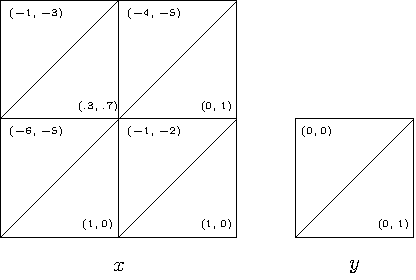
\includegraphics[width=.8\textwidth]{images/2014-2015-resit-img01.pdf}
        \end{center}

        \hfill[16]

    \end{enumerate}

\end{enumerate}

\makeatletter
\renewcommand{\@oddfoot}{\hfil \arabic{page}X \hfil}    % sets last page footer
\makeatother

\end{document}
